% vim: ts=4 sts=4 sw=4 et tw=75
\chapter{Algorithms and Data Structures}
\label{chap:alds}
\begin{quote}
    In the end, only familiarity with the tools and techniques of the field
    will provide right solution for a particular problem, and only a
    certain amount of experience will provide consistently professional
    result.
\end{quote}
\begin{quotesrc}
    Raymond Fielding.\bookname{The Technique of Special Effects
    Cinematography}
\end{quotesrc}
The study of algorithms and data structures is one of the foundations of
computer science, a rich field elegant (一流的) techniques and
sophisticated (老成的) mathematical analyses. And it's more than just fun
and games for the theoretically inclined: a good algorithm or data
structure might make it possible to solve a problem in seconds that could
otherwise take years.

In specialized areas like graphics, databases, parsing, numerical analysis,
and simulation, the ability to solve problems depends critically on
state-of-the-artalgorithms and data structures. If you are developing your
programs in a field that's new to you, you \textbf{\textit{must}} find out
what is already known, lest (免得) you waste your time doing poorly what
others have already done well.

Every program depends on algorithms and data structures, but few programs
depend on the invention of brand new ones. Even within an intricate
(错综复杂的) program like a compiler or a web browser, most of the data
structures are arrays, lists, trees and hash tables. When a program needs
something more elaborate(详细), it will likely be based on these simpler
ones. Accordingly, for most programmers, the task is to know what
appropriate algorithms and data structures are available and to understand
how to choose among alternatives.

Here is the story in a nutshell. There are only a handful of basic
algorithms that show up in almost every program -- primarily searching and
sorting -- and even those are often included in libraries. Similarly,
almost every data structure is derived (起源) from a few fundamental ones.
Thus the material covered in this chapter will be familiar to almost all
programmers. We have written working versions to make the discussion
concrete, and you can lift code verbatim (逐字的) if necessary, but do so
only after you have investigated what the programming language and its
libraries have to offer.

\section{Searching}
\label{sec:searching}
Nothing beats an array for storing static tabular data. Compile-time
initialization makes it cheap and easy to construct such arrays. (In Java,
the initialization occurs at run-time, but this is an unimportant
implementation detail unless the arrays are large.) In a program to detect
words that are used rather too much in bad prose, we can write
\begin{wellcode}
    char *flab[] = {
        "actually",
        "just",
        "quite",
        "really",
        NULL
    };
\end{wellcode}
The search routines needs to know how many elements are in the array. One
way to tell it is to pass length as an argument; another, used here, is to
place a \verb'NULL' marker at the end of the array:
\begin{wellcode}
    /* lookup: sequential search for word in array */
    int lookup(char *word, char *array[])
    {
        int i;
        for (i = 0; array[i] != NULL; i++)
           if (strcmp(word, array[i]) == 0)
                return i;
        return -1;
    }
\end{wellcode}
In C and C++, a parameter that is an array of strings can be declared as
\verb"char *array[]" or \verb"char **array". Although these forms are
equivalent, the first makes it clearer how the parameter will be used.

This search algorithm is called \textbf{\textit{sequential search}} because
it looks at each element in turn to see if it's the desired one. When the
amount of data is small, sequential search is fast enough. There are
standard library routines to do sequential search for specific data types;
for example, functions like \texttt{strchr} and \texttt{strstr} search for
the first instance of a given character or substring in a C or C++ string.
The Java \verb'String' class has an \verb'indexOf' method, and the generic
C++ \verb'find' algorithms apply to most data types. If such a function
exists for the data type you've got, use it.

Sequential search is easy but the amount of work is directly proportional
(成比例的)
to the amount of data to be searched; doubling the number of elements will
double the time to search if the desired item is not present. This is a
linear relationship -- run-time is a linear function of data size -- so
this method is also known as \textbf{\textit{linear search}}.

Here's an excerpt (引用) from an array of more realistic size from a
program that
parses HTML, which defines textual names for well over a hundred individual
characters:
\begin{wellcode}
    typedef struct Nameval Nameval;
    struct Nameval{
        char *name;
        int value;
    };
    /* HTML characters, e.g. AElig is ligature of A and E. */
    /* Values are Unicode/ISO10646 encoding. */
    Nameval htmlchars[] = {
        "AElig",    0x00c6,
        "Aacute",   0x00c1,
        "Acirc",    0x00c2,
        /* ... */
        "zeta",     0x03b6,
    };
\end{wellcode}

For a larger array like this, it's more efficient to use
\textit{binary} search. The binary search algorithm is an orderly
version of the way we look up words in a dictionary. Check the middle
element. If that value is bigger than what we are looking for, look in the
first half; otherwise, look in the second half. Repeat until the desired
item is found or determined not to be present.

For binary search, the table must be sorted, as it is here (that's good
style anyway; people find things faster in sorted tables too), and we must
know how long the table is. The \verb'NELEMS' macro from Chapter
\ref{chap:style} can help:
\begin{wellcode}
    printf("The HTML table has %d words\n", NELEMS(htmlchars));
\end{wellcode}

A binary search function for this table might look like this:
\begin{wellcode}
    /* lookup: binary search for name in tab; return index */
    int lookup(char *name, NameVal tab[], int ntab)
    {
        int low, high, mid, cmp;
        low = 0;
        high = ntab - 1;
        while (low <= high){
            mid = (low + high)/2;
            cmp = strcmp(name, tab[mid].name);
            if (cmp < 0){
                high = mid - 1;
            }
            else if (cmp > 0){
                low = mid + 1;
            }
            else{   /* found match */
                return mid;
            }
        }
        return -1;  /* no match */
    }
\end{wellcode}
Putting all this together, to search \verb'htmlchars' we write
\begin{wellcode}
    half = lookup("frac12", htmlchars, NELEMS(htmlchars));
\end{wellcode}
to find the array index of the character $1/2$.

Binary search eliminates half the data at each step. The number of steps is
therefore proportional to the number of times we can divide $n$ by 2
before we're left with a single element. Ignoring roundoff, this is
$\log_2n$.
If we have 1000 items to search, linear search takes up to 1000 steps,
while binary search takes about 10; if we have a million items, linear
takes a million steps and binary takes 20. The more items, the greater the
advantage of binary search. Beyond some size of input (which varies with
the implementation), binary search is faster than linear search.

\section{Sorting}
\label{sec:sorting}
Binary search works only if the elements are sorted. If repeated searches
are going to be made in some data set, it will be profitable to sort once
and then use binary search. If the data set is known in advance, it can be
sorted when the program is written and built using compile-time
initialization. If not, it must be sorted when the program is run.

One of the best all-round sorting algorithms is quicksort, which was
invented in 1960 by C. A. R. Hoare. Quicksort is a fine example of how to
avoid extra computing. It works by partitioning an array into little and
big elements:\\

\indent \indent pick one element of the array (the "pivot").
\\
\indent \indent partition the other elements into two groups:
\\
\indent \indent \indent "little ones" that are less than the pivot value,
and   \\
\indent \indent \indent "big ones" that are greater than or equal to the
pivot value.  \\
\indent \indent recursively sort each group.\\ \\
When this process is finished, the array is in order. Quicksort is fast
because once an element is known to be less than the pivot value, we don't
have to compare it to any of the big ones; similarly, big ones are not
compared to little ones. This makes it much faster than the simple sorting
methods such as insertion sort and bubble sort that compare each element
directly to all the others.

Quicksort is practical and efficient; it has been extensively studied and
myriad variations (各式变种) exist. The version that we present here is
just about the simplest implementation but it is certainly not the
quickest.

This \verb'quicksort' function sorts an array of integers:
\begin{wellcode}
    /* quicksort: sort v[0]..v[n-1] into increasing order */
    void quicksort(int v[], int n)
    {
        int i, last;
        if(n <= 1) /* nothing to do */
            return;
        swap(v, 0, rand() % n); /* move pivot elem to v[0] */
        last = 0;
        for(i = 1; i < n; i++)  /*partition */
            if(v[i] < v[0])
                swap(v, ++last, i);
        swap(v, 0, last);   /* restore pivot */
        quicksort(v, last); /* recursively sort */
        quicksort(v + last + 1, n - last - 1); /* each part */
    }
\end{wellcode}

The \verb'swap' operation, which interchanges two elements, appears three
times in \verb'quicksort', so it is best made into a separate function:
\begin{wellcode}
    /* swap: interchange v[i] and v[j] */
    void swap(int v[], int i, int j)
    {
        int temp;
        temp = v[i];
        v[i] = v[j];
        v[j] = temp;
    }
\end{wellcode}

Partitioning selects a random element as the pivot, swaps it temporarily to
the front, then sweeps through the remaining elements, exchanging those
smaller than the pivot ("little ones") towards the beginning (at location
\verb'last') and big ones towards the end (at location \verb'i'), At the
beginning of the process, just after the pivot has been swapped to the
front, \verb'last=0' and elements \verb'i=1' through \verb'n-1' are
unexamined:
\begin{figure}[h]
    \centering
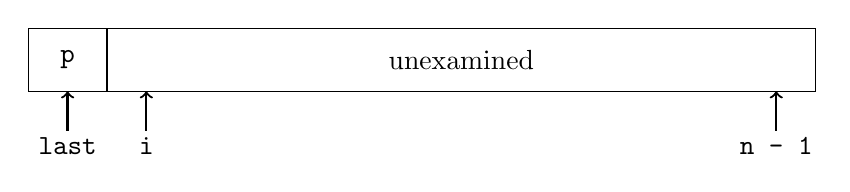
\begin{tikzpicture}
    \draw (0, 0) -- (10, 0);
    \draw (0, 0.8) -- (10, 0.8);
    \draw (0, 0) -- (0, 0.8);
    \draw (1, 0) -- (1, 0.8);
    \draw (10, 0) -- (10, 0.8);
    \node at(0.5, 0.4) {\verb'p'};
    \node at(5.5, 0.4) {unexamined};
    \draw[thick, ->] (0.5, -0.5) -- (0.5, 0);
    \draw[thick, ->] (1.5, -0.5) -- (1.5, 0);
    \draw[thick, ->] (9.5, -0.5) -- (9.5, 0);
    \node at(0.5, -0.7) {\texttt{last}};
    \node at(1.5, -0.7) {\texttt{i}};
    \node at(9.5, -0.7) {\texttt{n - 1}};
\end{tikzpicture}
\end{figure}\\
At the top of the \verb'for' loop, elements \verb'1' through \verb'last'
are strictly less than the pivot (中枢), elements \verb'last+1' through
\verb'i-1' are greater than or equal to the pivot, and elements \verb'i'
through \verb'n-1' have not been examined yet. Until \verb'v[i] >= v[0]',
the algorithm may swap \verb'v[i]' with itself; this wastes some time but
not enough to worry about.
\begin{center}
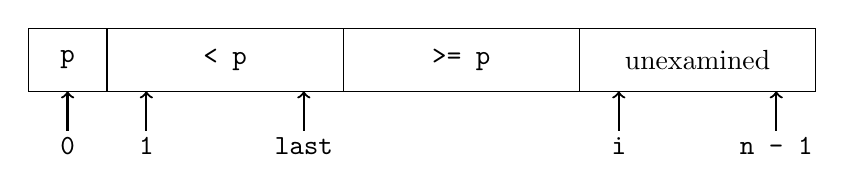
\begin{tikzpicture}
    \draw (0, 0) -- (10, 0);
    \draw (0, 0.8) -- (10, 0.8);
    \draw (0, 0) -- (0, 0.8);
    \draw (1, 0) -- (1, 0.8);
    \draw (4, 0) -- (4, 0.8);
    \draw (7, 0) -- (7, 0.8);
    \draw (10, 0) -- (10, 0.8);
    \node at(0.5, 0.4) {\verb'p'};
    \node at(2.5, 0.4) {\verb'< p'};
    \node at(5.5, 0.4) {\verb'>= p'};
    \node at(8.5, 0.4) {unexamined};
    \draw[thick, ->] (0.5, -0.5) -- (0.5, 0);
    \draw[thick, ->] (1.5, -0.5) -- (1.5, 0);
    \draw[thick, ->] (3.5, -0.5) -- (3.5, 0);
    \draw[thick, ->] (7.5, -0.5) -- (7.5, 0);
    \draw[thick, ->] (9.5, -0.5) -- (9.5, 0);
    \node at(0.5, -0.7) {\texttt{0}};
    \node at(1.5, -0.7) {\texttt{1}};
    \node at(3.5, -0.7) {\texttt{last}};
    \node at(7.5, -0.7) {\texttt{i}};
    \node at(9.5, -0.7) {\texttt{n - 1}};
\end{tikzpicture}
\end{center}
After all elements have been partitioned, element \verb'0' is swapped with
the \verb'last' element to put the pivot element in its final position;
this maintains the correct ordering. Now the array looks like this: \\
\begin{center}
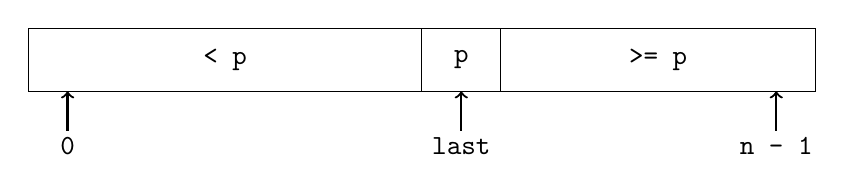
\begin{tikzpicture}
    \draw (0, 0) -- (10, 0);
    \draw (0, 0.8) -- (10, 0.8);
    \draw (0, 0) -- (0, 0.8);
    \draw (5, 0) -- (5, 0.8);
    \draw (6, 0) -- (6, 0.8);
    \draw (10, 0) -- (10, 0.8);
    \node at(2.5, 0.4) {\verb'< p'};
    \node at(5.5, 0.4) {\verb'p'};
    \node at(8, 0.4) {\verb'>= p'};
    \draw[thick, ->] (0.5, -0.5) -- (0.5, 0);
    \draw[thick, ->] (5.5, -0.5) -- (5.5, 0);
    \draw[thick, ->] (9.5, -0.5) -- (9.5, 0);
    \node at(0.5, -0.7) {\texttt{0}};
    \node at(5.5, -0.7) {\texttt{last}};
    \node at(9.5, -0.7) {\texttt{n - 1}};
\end{tikzpicture}
\end{center}

The same process is applied to the left and right sub-arrays; when this has
finished, the whole array has been sorted.

How fast is quicksort? In the best possible case,
\begin{itemize}
\item the first pass partitions $n$ elements into two groups of about $n/2$
    each.
\item the second level partitions two groups, each of about $n/2$ elements,
    into four groups each of about $n/4$.
\item the next level partitions four groups of about $n/4$ into eight of
    about $n/8$.
\item and so on.
\end{itemize}

This goes on for about $\log_2 n$ levels, so the total amount of work in
the best case is proportional to $n + 2\times n/2 + 4\times n/4 + 8\times
n/8 ... $ ($\log_2 n$ terms), which is $n\log_2 n$. On the average, it does
only a little more work. It is customary to use base 2 logarithms; thus we
say that quicksort takes time proportional to $n\log n$.

This implementation of quicksort is the clearest for exposition, but it has
a weakness. If each choice of pivot splits the element values into two
nearly equal groups, our analysis is correct, but if the split is uneven
too often, the run-time can grow more like $n^2$. Our implementation uses a
random element as the pivot to reduce the chance that unusual input data
will cause too many uneven splits. But if all the input values are the
same, our implementation splits off only one element each time and will
thus run in time proportional to $n^2$.

The behavior of some algorithms depends strongly on the input data.
Perverse or unlucky inputs may cause an otherwise well-behaved algorithm to
run extremely slowly or use a lot of memory. In the case of quicksort,
although a simple implementation like ours might sometimes run slowly, more
sophisticated implementations can reduce the chance of pathological
behavior to almost zero.


\section{Libraries}
\label{sec:libraries}
The standard libraries for C and C++ include sort functions that should be
robust against adverse inputs, and tuned to run as fast as possible.

Library routines are prepared to son any data type, but in return we must
adapt to their interface, which may be somewhat more complicated than what
we showed above. In C, the library function is named \verb'qsort', and we
need to provide a comparison function to be called by \verb'qsort' whenever
it needs to compare two values. Since the values might be of any type, the
comparison function is handed two \texttt{void *} pointers to the data items
to be compared. The function casts the pointers to the proper type,
extracts the data values, compares them, and returns the result (negative,
zero, or positive according to whether the first value is less than, equal
to, or greater than the second).

Here's an implementation for sorting an array of strings, which is a common
case. We define a function \verb'scmp' to cast the arguments and call
\verb'strcmp' to do the comparison.

\begin{wellcode}
    /* scmp: string compare of *p1 and *p2 */
    int scmp(const void *p1, const void *p2)
    {
        char *v1, *v2;
        v1 = *(char **) p1;
        v2 = *(char **) p2;
        return strcmp(v1, v2);
    }
\end{wellcode}
We could write this as a one-line function, but the temporary variables
make the code easier to read.

We can't use \verb'strcmp' directly as the comparison function because
\verb'qsort' passes the address of each entry in the array, \verb'&str[i]'
(of type \verb'char**'), not \verb'str[i]' (of type \verb'char*'), as shown
in this figure:
\begin{figure}[h]
    \centering
    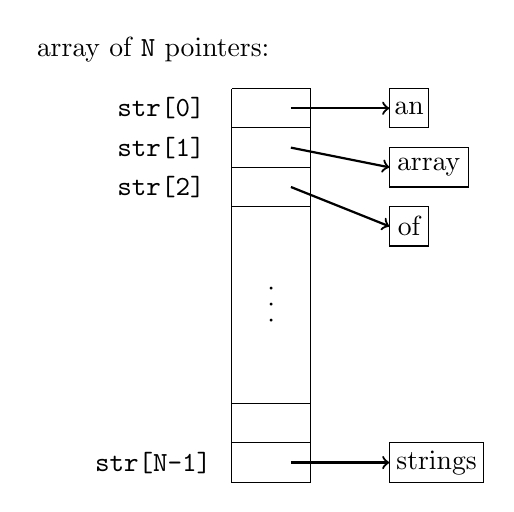
\begin{tikzpicture}
    \node at(0, 0.5) {array of \verb'N' pointers:};
    \draw (1, 0) -- (1, -5) -- (2, -5) -- (2, 0) -- (1, 0);
    \draw (1, -0.5) -- (2, -0.5);
    \draw (1, -1) -- (2, -1);
    \draw (1, -1.5) -- (2, -1.5);
    \draw (1, -4) -- (2, -4);
    \draw (1, -4.5) -- (2, -4.5);
    \node at(0.1, -0.25) {\verb'str[0]'};
    \node at(0.1, -0.75) {\verb'str[1]'};
    \node at(0.1, -1.25) {\verb'str[2]'};
    \node at(0, -4.75) {\verb'str[N-1]'};
    \draw[thick, ->] (1.75, -0.25) -- (3, -0.25);
    \node at(3.25, -0.25) {an};
    \draw (3, 0) -- (3, -0.5) -- (3.5, -0.5) -- (3.5, 0) -- (3, 0);
    \draw[thick, ->] (1.75, -0.75) -- (3, -1);
    \node at(3.5, -1) {array};
    \draw (3, -0.75) -- (3, -1.25) -- (4, -1.25) -- (4, -0.75) -- (3,
    -0.75);
    \draw[thick, ->] (1.75, -1.25) -- (3, -1.75);
    \node at(3.25, -1.75) {of};
    \draw (3, -1.5) -- (3, -2) -- (3.5, -2) -- (3.5, -1.5) -- (3, -1.5);
    \draw[thick, ->] (1.75, -4.75) -- (3, -4.75);
    \node at(3.6, -4.75) {strings};
    \draw (3, -4.5) -- (3, -5) -- (4.2, -5) -- (4.2, -4.5) -- (3, -4.5);
    \node at(1.5, -2.75) {$\cdot$};
    \node at(1.5, -2.55) {$\cdot$};
    \node at(1.5, -2.95) {$\cdot$};
    \end{tikzpicture}
\end{figure}\\
To sort elements \verb'str[O]' through \verb'str[N-l]' of an array of
strings, \verb'qsort' must be called with the array, its length, the size
of the items being sorted, and the comparison function:
\begin{wellcode}
    char *str[N];
    qsort(str, N, sizeof(str[0]), scmp);
\end{wellcode}

Here's a similar function \verb'icmp' for comparing integers:
\begin{wellcode}
    /* icmp: integer compare of *p1 and *p2 */
    int icmp(const void *p1, const void *p2)
    {
        int v1, v2;
        v1 = *(int *) p1;
        v2 = *(int *) p2;
        if (v1 < v2)
            return -1;
        else if (v1 == v2)
            return 0;
        else
            return 1;
    }
\end{wellcode}
We could write
\begin{badcode}
    return v1 - v2;
\end{badcode}
but if \verb'v2' is large and positive and \verb'v1' is large and negative
or vice versa (反过来), the resulting overflow would produce an incorrect
answer. Direct comparison is longer but safe.

Again, the call to \verb'qsort' requires the array, its length, the size of
the items being sorted, and the comparison function:
\begin{wellcode}
    int arr[N];
    qsort(arr, N, sizeof(arr[0]), icmp);
\end{wellcode}

ANSI C also defines a binary search routine, \verb'bsearch'. Like
\verb'qsort', \verb'bsearch' requires a pointer to a comparison function
(often the same one used for \verb'qsort'); it returns a pointer to the
matching element or \verb'NULL' if not found. Here is our HTML
\verb'lookup' routine, rewritten to use \verb'bsearch':
\begin{wellcode}
    /* lookup: use bsearch to find name in tab, return index*/
    int lookup(char *name, Nameval tab[], int ntab)
    {
        Nameval key, *np;
        key.name = name;
        key.value = 0;  /* unused; anything will do*/
        np = (Nameval *) bsearch(&key, tab, ntab, sizeof(tab[0]), nvcmp);
        if(np == NULL)
            return -1;
        else
            return np - tab;
    }
\end{wellcode}

As with \verb'qsort', the comparison routine receives the address of the
items to be compared, so the key must have that type; in this example, we
need to construct a fake \verb'Nameval' entry that is passed to the
comparison routine. The comparison routine itself is a function
\verb'nvcmp' that compares two \verb'Nameval' items by calling
\verb'strcmp' on their string components, ignoring their values:
\begin{wellcode}
    /* nvcmp: compare two Nameval names */
    int nvcmp(const void *va, const void *vb)
    {
        const Nameval *a, *b;
        a = (Nameval *) va;
        b = (Nameval *) vb;
        return strcmp(a->name, b->name);
    }
\end{wellcode}
This is analogous (相似) to \verb'scmp' but differs because the strings are
stored as members of a structure.

The clumsiness(笨拙) of providing the key means that \verb'bsearch'
provides less leverage(杠杆作用) than \verb'qsort'. A good general-purpose
sort routine takes a page or two of code, while binary search is not much
longer than the code it takes to interface to \verb'bsearch'. Nevertheless,
it's a good idea to use \verb'bsearch' instead of writing your own. Over
the years, binary search has proven surprisingly hard for programmers to
get right.

The standard C++ library has a generic algorithm called \verb'sort' that
guarantees $O(n\log n)$ behavior. The code is easier because it needs no
casts or element sizes, and it does not require an explicit comparison
function for types that have an order relation.
\begin{wellcode}
    int arr[N];
    sort(arr, arr + N);
\end{wellcode}
The C++ library also has generic binary search routines, with similar
notational advantages.
\begin{exercise}
Quicksort is most naturally expressed recursively. Write it iteratively and
compare the two versions. (Hoare describes how hard it was to work out
quicksort iteratively, and how neatly it fell into place when he did it
recursively.)
\end{exercise}

\section{A Java Quicksort}
\label{sec:a_java_quicksort}
